%% pubi
%% Environmental Management
%% JASSS


\documentclass{article}
\usepackage[utf8]{inputenc}
\usepackage{authblk}
\usepackage[margin=1.25in]{geometry}
\usepackage{graphicx}
\usepackage{subcaption} % Allows the use of subfigures and subcaptions within figures
%\usepackage{amsmath} % Provides advanced mathematical typesetting features
\usepackage{lineno} % Enables the inclusion of line numbers in the document
\usepackage{booktabs} % Enhances the quality of tables, particularly those generated from R
\usepackage{makecell} % Provides better control over table cell formatting
\usepackage{hyperref} % Combined with biblatex it create link with biblio

\linenumbers

%%%%%% Bibliography %%%%%%

\usepackage[
    style=nejm, 
    citestyle=authoryear-ibid,
    sorting=none,
    mincitenames=1,
    maxcitenames=2, 
    backend=biber]{biblatex}

\addbibresource{treeModel.bib}

%%%%%% Title %%%%%%
% Full titles can be a maximum of 100 characters, including spaces. 
% Title Format: Use title case, capitalizing the first letter of each word, except for certain small words, such as articles and short prepositions
\title{From Local Actors to Leaf Protectors: A Companion Modeling Approach for Rethinking Tree Management and Protection Measures in Senegal's Groundnut Basin}

%%%%%% Authors %%%%%%
% Authors should be listed in order of contribution to the paper, by first name, then middle initial (if any), followed by last name.
% Authors should be listed in the order in which they will appear in the published version if the manuscript is accepted. 
% Use an asterisk (*) to identify the corresponding author, and be sure to include that person’s e-mail address. Use symbols (in this order: †, ‡, §, ||, ¶, #, ††, ‡‡, etc.) for author notes, such as present addresses, “These authors contributed equally to this work” notations, and similar information.
% You can include group authors, but please include a list of the actual authors (the group members) in the Supplementary Materials.
\author[1,2,6*$\dag$]{E. Delay}
\author[1,2,4$\dag$]{L. Broutin}
\author[1,2]{A. Fallot}
\author[3]{A. Perrotton}
\author[4]{A. Gonin}
\author[5]{D. Masse}


%%%%%% Affiliations %%%%%%
\affil[1]{CIRAD, UMR SENS, F-34398 Montpellier, France.}
\affil[2]{SENS, CIRAD, IRD, Université de Paul Valéry Montpellier 3, Montpellier, France.}
\affil[3]{Forêts et Sociétés, Univ Montpellier, CIRAD, Montpellier, France.}
\affil[4]{Université Paris Nanterre, Laboratoire LAVUE, FR.}
\affil[5]{IRD, Eco\&Sols, Abidjan, Côte d’Ivoire.}
\affil[6]{UMI UMMSCO,  Université Cheick Anta Diop, Dakar, Sénégal.}
\affil[*]{Address correspondence to: etienne.delay@cirad.fr}
\affil[$\dag$]{These authors contributed equally to this work.}

%%%%%% Date %%%%%%
% Date is optional
\date{}


\begin{document}

\maketitle

%%%%%% Abstract %%%%%%
\begin{abstract}

    How can a participatory simulation model contribute to understanding the socio-ecological dynamics and fostering innovative strategies for sustainable management of trees, crops, and pastoralism in the peanut basin?

    In the agro-pastoral zones, the Sahelian ecosystems have undergone significant degradation, characterized by a reduction in tree cover, as a consequence of the droughts in the 1960s and 1990s. The peanut basin stands out for its positive interrelationships between trees, crops, and pastoralism. However, the regeneration of the Faidherbia park has declined since the major droughts. Through collaborative efforts with agro-pastoral farmers, we have developed a simulation model -- The SAFIRe model : Simulation of Agents for Fertility, Integrated Energy, Food security, and Reforestation-- that aims to unravel the complex social and ecological dynamics at play and explore potential strategies in partnership with local communities.

    By exploring the results of the model co-designed with local stakeholders, we have identified more effective management strategies, as per the request of the local actors. However, more importantly, we have collectively questioned the conditions for improving tree cover and the viability of the socio-ecosystem, particularly in relation to the demand for firewood and local cereal for sustenance. This has prompted the stakeholders to engage in community-wide discussions and transform agro-pastoralists into leaf protectors.

\end{abstract}

%%%%%% Main Text %%%%%%

\section{Introduction}

The Sahelian region has witnessed a series of devastating droughts from the 1960s to the 1990s, leading to substantial ecosystem degradation, particularly through a significant reduction in tree cover \parencite{mbow_what_2015}. This loss has adversely affected essential ecosystem services, impacting both the population and biodiversity. The severity of this tree cover loss becomes even more alarming given the rapid population growth in the Sahelian region \parencite{cesaro_reforestation_2023}. In a context of scarcity, intensive natural resource utilization by agriculture and livestock further exacerbates land degradation and soil fertility \parencite{tappan_landscapes_2016}.

Ester Boserup \parencite{boserup_conditions_1965} proposed that declining soil fertility compels farmers to intensify their agricultural practices. Subsequent studies have often focused on this intensification as a primary response to social and agricultural phenomena.

Within the DSCATT project (Dynamics of Carbon Sequestration in Soils of Tropical and Temperate Agricultural Systems), participants in Senegal's living-labs quickly associated soil fertility with the presence of \textit{Faidherbia albida} trees. This insight directed our research towards understanding the significance of trees in the agricultural practices of the Senegalese peanut basin. By examining tree usage and local management practices, we developed the SAFIRe model (Simulation of Agents for Fertility, Integrated Energy, Food Security, and Reforestation). This approach is part of Companion Modeling (ComMod) \parencite{etienne_companion_2014, barreteau_our_2003} and Accompanying Exploration (ComExp) \parencite{delay_comexp_2020}, aiming to collaboratively explore potential futures for the territory.

In the context of sustainable land management, restoration options identified by farmers are closely linked to tree monitoring to mitigate predation risks from neighboring populations, especially in the longstanding conflict between farmers and herders. Two exploration pathways emerged from discussions with local communities: the impact of delegated surveillance to forestry agents and the conditions for tree park development under community-managed surveillance.

We thus explored community-based natural resource conservation solutions, extensively documented since the Rio Summit promoted them \parencite{selfa_politics_2008, maraseni_assessment_2019, he_community_2020}. While the influence of different tree management approaches (delegated to forestry services or managed by the community) has been extensively debated, highlighting the territorial configurations each approach generates, a crucial point was raised. Through our co-constructed agent-based simulation, validated by stakeholders, we demonstrated that herders were often scapegoated for tree loss in the area. As farmers transitioned from manual to plough-based agriculture, they did not have time to adapt their practices to protect young tree saplings.

By employing ComMod and ComExp approaches, we aimed to assist stakeholders in reimagining future scenarios \parencite{jansujwicz_localism_2021} to support desired territorial transformation. Our goal here is to facilitate discussions and enhance stakeholders' capabilities through companion modeling. By adopting "Different Modelling Purposes" \parencite{edmonds_different_2019}, we position our intervention within two categories: illustration and social learning \parencite{sukthankar_kilt_2017}. We view illustration as a means to discern viable paths by extensively exploring the co-constructed model. These illustrations should remain within a framework of social learning, meaning they are constructed to reflect the shared vision of stakeholders about the world, assuming that they will then be better positioned to leverage the results to transform their system.

\section{Materials and Methods}

The Rio Summit in 1992 marked a significant turning point in the perception of natural resource management. It contributed to the democratization of community-based management, promoting a shift from an authoritarian vision of resource management to more integrated approaches \parencite{delay_coming_2022}. This evolution recognized the importance of actively involving local stakeholders in decision-making and the management of their natural environments. However, integrating communities into resource management processes has introduced complex challenges, particularly regarding the co-construction of common representations and understandings of these environments.

Integrating heterogeneous actors within collectives to co-construct models and simulations has emerged as an innovative response to these challenges. Fully aligned with the philosophy of companion modeling, this approach has given rise to novel methods. In our work, we facilitated workshops aimed at developing an anticipatory method we named ACARDI \parencite{perrotton_definition_2021}. This method relies on close collaboration between researchers and local actors, emphasizing the co-construction of models and simulations to anticipate territorial changes. At the end of the process, we established the first Living Lab of the Niakhar observatory.

After conducting participatory workshops in Diohine, actively involving local stakeholders, we identified several specific aspirations and concerns of the population regarding their territory. Among these, the aspiration for the "return of fauna and flora" particularly caught our attention. To explore this aspiration more thoroughly, we combined an anthropological approach with the co-construction of a simulation model. This section focuses on our approach and methodology aimed at bringing this aspiration to life, combining socio-cultural aspects and modeling tools for a holistic understanding.

\subsection{Modelling for Empowerment - An Anthropological Approach to Participatory Model Co-construction}

The implementation of the ACARDI workshops marked a crucial phase of our research, characterized by a three-month immersion in Diohine. This immersion extended beyond workshop discussions, enabling an in-depth information collection process through interviews and participant observation. This fieldwork was essential for gaining a nuanced understanding of the local population's aspirations and concerns regarding territorial management.

Through these interviews, focus groupes and participant observation, a process of developing conceptual models was initiated, gradually evolving into the creation of an agent-based computational model. The co-construction of these models was a collaborative and iterative approach, actively involving the stakeholders of the Diohine Living Lab. Local actors played a key role in discussing, evaluating, and validating each aspect of the model, thereby ensuring it accurately reflected their realities and expectations.

Following a thorough validation of the model with local stakeholders, described as expert validation \parencite{bommel_definition_2009}, we began exploring the model using the OpenMole platform \parencite{reuillon_openmole_2013}. This exploration phase allowed us to simulate various scenarios and gather significant results, which were then presented to the Living Lab participants for feedback and further discussion. To facilitate this crucial step, we developed an interactive interface designed to simplify the manipulation and validation of large amounts of data by the stakeholders, ensuring a smooth and collaborative experience.

\subsection{ODD }

In this section, we will describe the SAFIRe model (Simulation of Agents for Fertility, Integrated Energy, Food security, and Reforestation) using the ODD (Overview, Design concepts, and Details) framework \parencite{grimm_standard_2006,grimm_odd_2010,grimm_odd_2020}.


    \subsubsection{Overview}

        \textbf{Purpose}

        The peanut basin is facing a loss of soil fertility. Chemical amendments are either unavailable in the area or economically inaccessible for farmers. Therefore, soil fertility depends on two aspects: the presence of livestock in the territory to maintain year-round manure, and the Faedherbia albida trees which play a fundamental role in crop cycles. Indeed, these trees have the unique characteristic of shedding their leaves during the growing season and fixing nitrogen from the air into the soil.

        The model thus aims to evaluate and explore solutions for managing the Faedherbia park to increase their density. The model focuses on exploring so-called community initiatives.

        The objective of this study was co-defined with the participants based on their desire to restore trees and biodiversity. According to their perspective, the decline in tree population is strongly linked to individual practices associated with pastoralism. Thus, the aim was to reassess the functioning of their system, the role of "tree cutters," and the optimization of surveillance by comparing community-based surveillance efforts with centralized surveillance conducted by them and the forestry department.\\

        Throughout the study, we also examined the role of farmers and agro-pastoralists in the disappearance of trees. It was observed that young tree seedlings are no longer marked and destroyed by animal-drawn tools.\\

        \textbf{Entities, state variables and scales}

        The entities in the model are relatively numerous: some are static (trees, plots, and village), while others are in motion (shepherds, farmers, woodcutters, and overseers). 

        patches : nbarbresici: Number of trees present on this patch; arbre-ici: Indicates if there is a tree on this patch (reference to a specific tree); tree-influence: Influence of the tree on this patch (can represent aspects like shade, nutrients affected by the tree, etc.); under-tree: (TRUE/FALSE) Indicates if the patch is under a tree; culture: Type of crop on this patch (can be millet or groundnut); en-culture: Indicates if the patch is currently used for crops; rendement-mil-g: Yield of millet on the patch in terms of grains (to be calibrated later); rendement-mil-p: Yield of millet on the patch in terms of bundles; rendement-groundnuts-g: Yield of groundnuts on the patch in terms of grains; rendement-groundnuts-p: Yield of groundnuts on the patch in terms of bundles; id-parcelle: Identifies the parcel, allowing the structure of the parcels to be maintained during rotation; pas-rotation: Tracks parcels that have not yet rotated (system of +1); rotation: (TRUE/FALSE) Indicates if the parcel has already undergone rotation; champ-brousse: Indicates if the patch is in bushland; zoné: (TRUE/FALSE) Indicates if the patch is used for defining fallow zones; zone: Indicates to which fallow rotation zone the patch belongs (there are 3 zones for fallow rotation).

        Trees : proche-village: Likely unnecessary variable (trees in villages are also pruned); nb-coupes: Number of cuts; nb-jour-coupe: Number of cutting days; age-tree: Age of the tree. Trees have olso a subclass Saplings composed by age: Age in days ; signalé: Reported; rna-coupe: Cut in RNA.


        farmers : id-agri: Links to the farmer's unique parcel; engagé: TRUE/FALSE engagement in the Assisted natural regeneration (RNA in fr); interet-RNA: Interest in the RNA; jour-champ: Days spent in the field; nb-ha-a: Number of hectares allocated; stock-mil: Stock of millet; idMyBerger: Identifier of the associated shepherd; nb-patches: Number of patches; mon-chp-RNA: Field in the RNA.


        hearder : troupeau-nourri: does the herd have enough to eat, currently TRUE/FALSE; arbre-choisi: tree chosen to be cut and fed to animals as fodder ; nb-têtes: herd size for the shepherd ; nb-ha-b: Between 3.8 (newly settled, 11\%) and ~5.5 (89\% of the population); stock-fourrage: Forage stock; idAgri: Identifier of my reference farmer.

        woodcutters : attrape: Captured (TRUE/FALSE); nb-attrape: Number time he was captured; jours-peur: Days of fear after capuration; en-coupe: Currently cutting.


        The simulated space, through which the agents interact, represents 100 hectares. It is composed of 1000 spatial entities (patches) with a size of 10 square meters (resolution). It is exclusively agricultural since the inhabited area of the village is condensed into a single point. (The areas that are not cultivated, such as wetlands and pathways, are rare and have not been represented.)

        The irreducible time step is one day (tick). The various elements of the system (interactions, etc.) take into account the seasonality that structures agricultural activities. Every 364 days, a new year begins and the rhythm of the seasons continues. A second time unit can be considered: the year, which consists of seasons. Simulations are generally carried out over 23 years. At the beginning of the simulation, the first 3 years are considered to initialize the model.\\
    
        \textbf{Process overview and scheduling}\\

        This section provides an overview of the processes and their scheduling within the model. The model is composed of several sub-models that simulate various aspects of the ecosystem and human activities. Each process is organized and executed in a specific sequence to reflect the interactions and dependencies within the system. The following describes repeated procedures that occur at each time step:

        \begin{itemize}
            \item Harvest and Crop Management
            \begin{itemize}
                \item Harvest and stockpiling: Farmers harvest crops and store them in their stockpiles.
                \item Effect of machinery on unprotected saplings: Machinery used in the fields may damage or destroy unprotected saplings.
                \item Crop rotation: Farmers rotate crops between different fields to maintain soil fertility and reduce pest buildup.
            \end{itemize}

            \item Tree Growth and Reproduction
            \begin{itemize}
                \item Sprouting: New saplings sprout around mature trees, influenced by tree density and environmental conditions.
                \item Sapling growth: Saplings grow over time, with growth rates dependent on available resources and environmental factors.
                \item Aging and death of trees: Trees age and may eventually die due to old age, disease, or other environmental factors.
            \end{itemize}

            \item Livestock Feeding and Forage Use of Acacias
            \begin{itemize}
                \item Feeding livestock with straw: Shepherds feed their livestock with straw collected from the fields.
                \item Tree cutting: Trees are cut down for forage or other uses by the shepherds.
                \item Livestock in fallow land and cutting of saplings: Livestock graze in fallow lands, and shepherds may cut down saplings to manage the land.
            \end{itemize}

            \item Cutting of Saplings by Woodcutters
            \begin{itemize}
                \item Detection of saplings: Woodcutters search for and identify saplings that can be cut.
                \item Cutting of saplings: Once identified, saplings are cut by the woodcutters for use as firewood or other purposes.
            \end{itemize}

            \item Farmer Engagement
            \begin{itemize}
                \item Participation in meetings: Farmers participate in community meetings to discuss agricultural practices and share knowledge.
                \item Observing the success of neighbors: Farmers observe the practices and successes of their neighbors to learn and adapt.
                \item Social interaction and motivation: Social interactions among farmers influence their motivation and engagement in community activities.
                \item Protection of saplings: Farmers take actions to protect saplings from damage by livestock or machinery.
            \end{itemize}

            \item Surveillance
            \begin{itemize}
                \item Surveillance and presence of farmers in the fields (generalized community surveillance): Farmers patrol their fields and monitor for any issues such as pests or unauthorized grazing.
                \item Delegated community surveillance: Specific individuals or groups are assigned the task of community surveillance to ensure all fields are monitored effectively.
            \end{itemize}
        \end{itemize}


    \subsubsection{Design Concepts}

        \textbf{Basic principles}\\

        In their paper \parencite{roupsard_how_2020}, a link was established between the presence of \textit{Faidherbia albida} trees and the improvement of crop yields in the region. We have extended this work to calibrate the model on the relationship between these trees and cultivated plants. By engaging with stakeholders on their interactions with plants through food and livestock, we aimed to socially address the paradox of the non-renewal of these trees. Given that the area has been well-documented by agronomists since the establishment of the Niakhar observatory, we were able to collect quantitative data on historical \parencite{pieri_fertilite_1989, pelissier_paysans_1966} and contemporary \parencite{audouin_chapitre_2018, ba_impact_2018} forms of rural organization. This comprehensive documentation facilitated our understanding and analysis of the agricultural systems and social structures within the region. This work primarily involved adopting a systemic approach as identified by the stakeholders during participatory modeling workshops using the ARDI methodology \parencite{etienne_ardi_2011,etienne_companion_2014}.\\

        % Which general concepts, theories, hypotheses, or modeling approaches are underlying the model’s design? Explain the relationship between these basic principles, the complexity expanded in this model, and the purpose of the study.

        \textbf{Adaptation}\\
        
        Two agents exhibit adaptive/changing behaviors: the woodcutters and the farmers. The response of the woodcutters to being caught by a sapling protector varies according to the number of times they have been caught previously. Farmers have a score describing their interest in tree protection. This score evolves constantly according to several rules: encountering another engaged farmer, observing the success of a neighbor's protection system, participating in meetings, etc.\\

        \textbf{Emergence}\\

        %What key results or outputs of the model are modeled as emerging from the adaptive traits, or behaviors, of individuals?

        There are several intriguing elements to examine, such as the emergence at the model level and the enhanced understanding of social and ecological interrelationships and solidarity among the actors. The model emphasizes the significant impact of agriculture (likely due to the introduction of plow-based farming) on the destruction of \textit{Faidherbia albida} saplings (weak emergence). Moreover, a strong emergence is observed when agents are permitted to organize on a community level, as neighbors gradually engage each other in sustaining interest in assisted tree regeneration.

        Highlighting potential long-term trajectories to reach acceptable production volumes should be considered both from the viewpoint of weak emergence within the model, due to its mechanistic processes, and strong emergence, as it drives participants to actively engage and commit to the theme beyond the facilitation process.\\


        \textbf{Sensing}\\

        %What internal and environmental state variables are individuals assumed to sense and consider in their decisions? 

        The patches within the action radius of the trees will yield more. Agents are capable of perceiving the farmers around them. Shepherds will not cut young saplings if there is a concerned farmer nearby, and the same applies to woodcutters. Farmers, in turn, perceive their neighbors and will interact with them if they have adjacent fields. Through these interactions, they discuss assisted natural regeneration (ANR) to persuade each other to adopt this practice.


        \textbf{Interaction}\\

        The interaction between agents is direct. Woodcutters interact directly with the saplings by cutting them down. Similarly, shepherds interact directly with the trees by utilizing them for forage. Farmers and supervisors also have direct interactions with woodcutters by stopping them from cutting the saplings. Additionally, farmers destroy young saplings that are not protected.

        \begin{itemize}
            \item \textbf{Woodcutters and Saplings}: Woodcutters seek out saplings and cut them down for use as firewood or other purposes. This direct interaction reduces the number of saplings in the environment.
            \item \textbf{Shepherds and Trees}: Shepherds interact with trees by feeding their livestock with tree foliage or cutting down trees for forage. This direct interaction affects the tree population and influences the availability of forage resources.
            \item \textbf{Farmers and Woodcutters}: Farmers interact with woodcutters by attempting to stop them from cutting saplings. When farmers encounter woodcutters in the field, they may intervene to protect the saplings.
            \item \textbf{Supervisors and Woodcutters}: Supervisors, acting as protectors, also interact directly with woodcutters. They monitor the fields and stop woodcutters from cutting down saplings to ensure the protection of young trees.
            \item \textbf{Farmers and Unprotected Saplings}: Farmers destroy young saplings that are not protected. This interaction occurs when farmers are working in their fields and come across unprotected saplings, which they remove to prevent interference with their crops.
        \end{itemize}

        \textbf{Stochasticity}\\

        Many events in the model rely on stochasticity since they are probabilistic. Probability is often used as a frequency measure. This is the case for the movements of farmers in their fields and the probability that farmers will discuss the RNA (Assisted natural regeneration) with each other.

        Stochasticity is used to represent uncertainty, particularly concerning whether supervisors catch woodcutters. Since supervisors do not spend the entire day in a single field, they may visit a field without encountering the woodcutter.

        Finally, randomness is used to create variability in initial conditions. This is the case for the number of heads in different herds, which vary in size, and for the initial age of each tree, resulting in trees of varying ages.

        \begin{itemize}
            \item Partial Randomness as Uncertainty
            \begin{itemize}
                \item Farmer Movements: The movements of farmers within their fields are determined randomly. This means that their location at any given time is based on a probability distribution, ensuring variability in their positions.
                \item Discussions about RNA: The likelihood that farmers will engage in discussions about the RNA is also probabilistic. This frequency-based probability allows for random interactions among farmers, influencing their engagement with the RNA.
                \item Supervisors and Woodcutters: The uncertainty in supervisors catching woodcutters is modeled using partial randomness. Supervisors patrol fields but may not always encounter woodcutters due to the random nature of their patrol routes and the woodcutters' activities.
            \end{itemize}

            \item Randomness for Initial Variability
            \begin{itemize}
                \item Herd Sizes: The initial number of heads in each herd is determined randomly, resulting in herds of varying sizes. This introduces variability into the model, reflecting real-world differences in herd sizes.
                \item Tree Ages: The initial age of each tree is assigned randomly, creating a population of trees with a range of ages. This variability in tree ages ensures a more realistic representation of a forest with trees at different stages of growth.\\
            \end{itemize}
        \end{itemize}

        \textbf{Collective actions}\\

        Collective forms emerge with the engagement of farmers in the protection of saplings. The larger the group of engaged farmers, the more likely it is for others to join, and the more assured the group's longevity.

        \begin{itemize}
            \item Farmer Engagement: As farmers begin to engage in sapling protection, they form groups that work collectively towards this goal.
            \item Group Growth: The probability of additional farmers joining the group increases with the group's size. This creates a positive feedback loop where the more farmers are engaged, the more likely it is for others to join.
            \item Group Longevity: The sustainability of the group is enhanced as it grows. A larger group of engaged farmers is more resilient and capable of maintaining their collective efforts over time.\\
        \end{itemize}


        \textbf{Observation}\\

        % What data are collected from the ABM for testing, understanding, and analyzing it, and how and when are they collected?

        We will monitor several metrics:

        \begin{itemize}
            \item Millet and Groundnut Production: This indicator tracks the total production of millet and groundnut in the simulation. It helps assess the agricultural output and food security within the modeled environment.
            \item Number of Trees at Each Development Stage: This metric measures the number of trees at various stages of development, such as saplings, young trees, and mature trees. It provides insight into the growth dynamics and regeneration of the forest.
            \item Number of Trees Destroyed by Each Type of Agent: This indicator counts the number of trees destroyed by different agents, such as farmers, woodcutters, and livestock. It helps understand the impact of various human and animal activities on the forest.
            \item Volume of Wood Cut for Cooking: This metric tracks the amount of wood harvested specifically for cooking purposes. It helps assess the pressure on forest resources for domestic energy needs.
            \item Age of Each Tree Sapling: This indicator measures the age of each sapling in the simulation. It provides information on the regeneration rate and the survival of young trees.
            \item Number of Farmers Engaged in the RNA: This metric tracks the number of farmers actively participating in the National Agricultural Network (RNA). It helps evaluate the level of community involvement and engagement in agricultural and environmental initiatives.\\
        \end{itemize}

    \subsubsection{Details}
        
        \textbf{Initialization}\\
        At initialization, the environment is generated with the following steps:

        \begin{itemize}
            \item Generation of Parcels and Crops: The landscape is divided into parcels, each designated for specific types of crops. This step sets up the agricultural fields and assigns crop types to each parcel.
            \item Generation of Trees and Their Fertilizing Effects: Trees are distributed throughout the environment, considering their effects on soil fertility. Trees influence the nutrient levels of the patches they occupy, enhancing soil quality in their vicinity.
            \item Generation of Human Agents: Human agents, including shepherds, woodcutters, farmers, and supervisors, are created and placed in the environment. Each agent type has specific roles and behaviors that contribute to the model's dynamics.
            \item Generation of the Village: The village is established as a central location where human agents reside. This step involves setting up the village infrastructure and assigning homes to the agents.
        \end{itemize}

        \textbf{Input data}\\

        We dont use input data.\\

        \textbf{Submodels}\\




\subsection{Statistical Analysis and our Companion Modeling approch}

Our work is grounded in the approach of companion modeling \parencite{barreteau_our_2003}. However, we aim to address the pressing need for model exploration. This entails combining and hybridizing elements that are rarely integrated: exploring the model alongside the stakeholders. To achieve this, we employed traditional agent-based modeling tools and made a concerted effort to conduct these analyses with the farmers of the peanut basin, engaging them in discussions about the exploration results. We performed a sensitivity analysis and utilized the "pattern space exploration" method to produce results reflecting the range of possible long-term scenarios. These results were then discussed with the stakeholders to ensure a comprehensive understanding and validation.

    \subsubsection{Sensitivity analysis : saltelli method}

    Sensitivity analysis comprises a range of techniques that assess how a model responds to variations in its input parameters. These statistical methods aim to quantify the extent to which changes in the inputs influence the variability observed in the outputs. In accordance with the definition provided by Saltelli et al. (2008)\parencite{saltelli_global_2008}, sensitivity analysis determines the "relative importance of each input in determining [output] variability." Consequently, these methods often yield a ranking or ordering of the inputs based on their respective sensitivity levels.\\

    \subsubsection{Pattern Space Exploration (PSE)}
    The PSE \parencite{cherel_beyond_2015}  method, based on genetic algorythme, is specifically designed to comprehensively cover the output space, resulting in its maximum score in output exploration -- e.g. "explore the output's diversity of a model"\footnote{\url{https://openmole.org/PSE.html}, consulté le 5 juin 2023}. By exploring the output space (c.f. fig. \ref{fig:PSE_explained}), the PSE method uncovers new patterns, providing insights into the model's sensitivity by examining the corresponding input values. Unlike calibration-based methods, PSE's effectiveness is influenced by the dimensionality of the output space, as it keeps a record of all the covered locations during exploration.

    \begin{figure}[h]
        \centering
        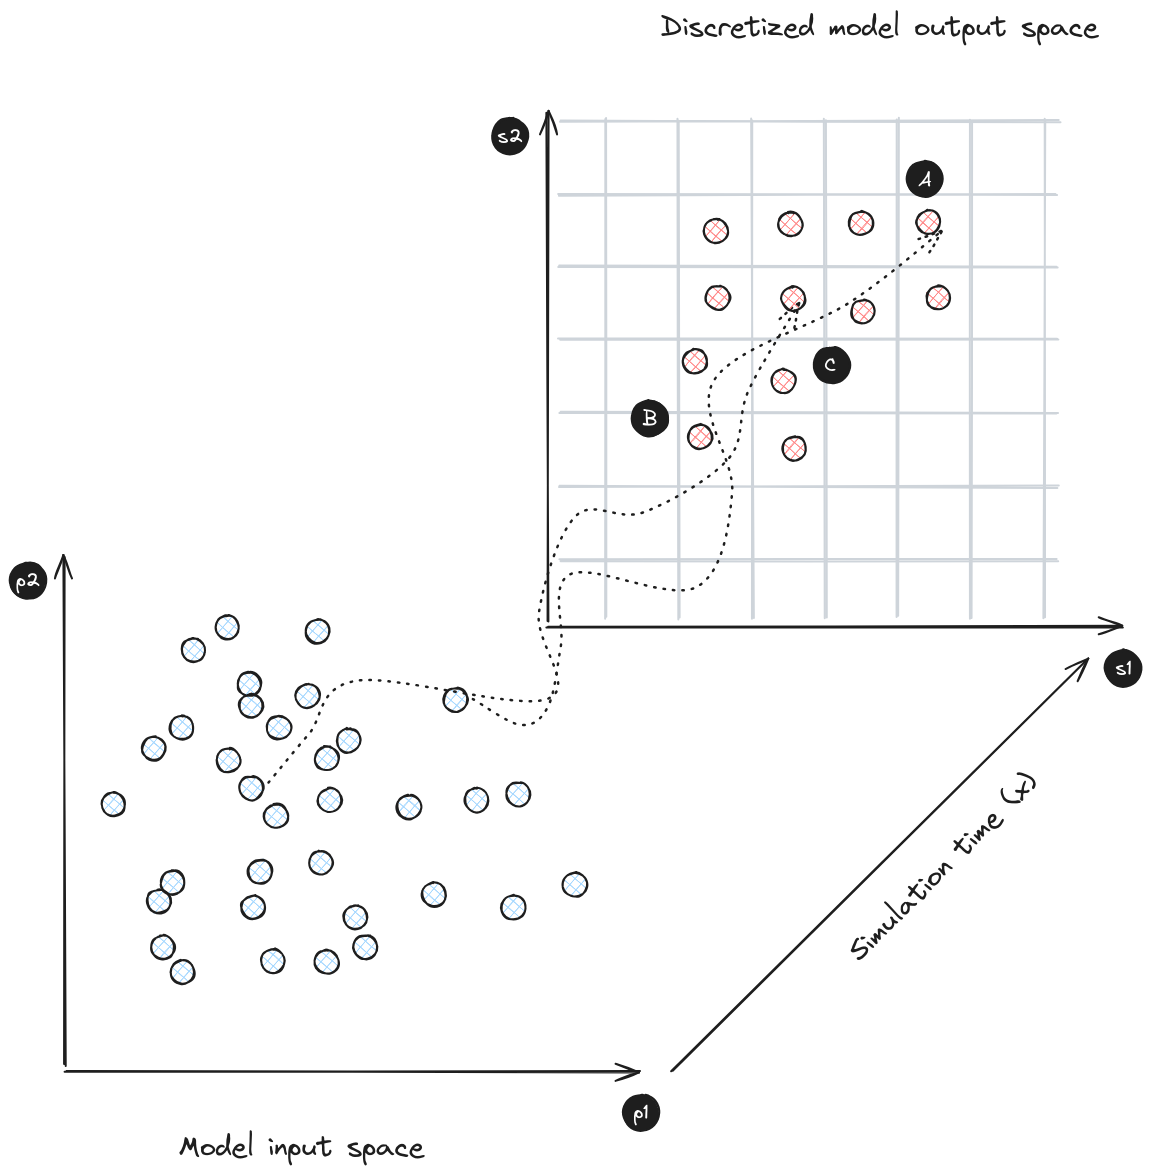
\includegraphics[width=\textwidth]{./img/pse_descritption.png}
        \caption{description of how the “pattern space exploration” genetic algorithm works. We see "p1" and "p2" as input parameters, and "s1" and "s2" as output parameters. The algorithm seeks to reach every cell in the grid of "s1" and "s2" to discover the model's output result domains. A and B and C are outputs of contrasting models}
        \label{fig:PSE_explained}
    \end{figure}
    

    In addition, the PSE method usually takes stochasticity into account by estimating selected models using the median of multiple output values obtained from model runs. For our purposes, and as we are in a situation where the results need to be discussed with stakeholders, we have chosen to focus not on the median, but on the last decille. This means that simulations are retained if more than 90\% of the results converge towards the identified output.

    The algorithm's ability to explore a diversity of output forms is extraordinarily powerful in the context of companion modeling. Indeed, participants in co-construction sessions gradually became accustomed to the practice of modeling \parencite{etienne_companion_2014}. They developed the ability to interrelate various elements of the system. However, the strength of agent-based modeling lies in the fact that they cannot anticipate emergent phenomena. Once the model has gained sufficient confidence, questioning the group about marginal aspects or unconsidered input parameter sets in the model proves to be extremely fruitful from the perspectives of emancipation and anticipating unforeseeable situations.

    \subsubsection{Engaging Stakeholders in Result and Thresholds Discussions}

    Working with participants on the PSE results enabled us to address the final conditions and thus the various configurations of the future. To facilitate this, we organized a feedback workshop during which we presented the simulation outcomes and discussed their implications for the systems they had described.

    Subsequently, we took time for collective reflection during which the participants collaboratively defined the final conditions that seemed particularly compelling to them. This interest was formalized around contrasting models.

    These archetype outputs allowed us to address and clarify situations that were previously unthinkable \parencite{banos_simulation_2010}. On figure \ref{fig:PSE_explained}, we can perceive situations A, B, and C as a series of contrasting scenarios for which we will discuss with the participants the configurations that have led to these outcomes. This leads to extremely rich discussions that compel stakeholders to consider these previously unthinkable situations and to collectively discuss the processes for satisfying individual needs regarding the collective inputs.


\section{Results}

The Saltelli analysis allows us to compare two surveillance scenarios, enabling us to identify the rearrangement of variables that occurs when the surveillance regime changes.

Following this, we conducted a Pattern Space Exploration (PSE) to identify the simulations that, in the context of community surveillance, increase the number of trees. This is a nonlinear process with an increase in fertility correlated with an increase in the number of trees.


    \subsection{Understanding stackolders Variable Importance via Sensitivity Analysis}

    We conducted the same analysis twice on different simulation scenarios. First, we performed an analysis on the community surveillance system. The second analysis shifts the workload to a dedicated surveillance system to mimic the functioning of surveillance by a water and forest authority.

    Comparing these two analyses allows us to assess the influence of a change in practice on the system's operation and to identify the structural changes they induce.

    In a community surveillance scenario, the global sensitivity analysis shows that the probability of discussing the importance of trees plays an extremely significant role in both millet production ($0.72$) and the total number of trees ($0.59$) at the end of the simulation (see Table \ref{tab:saltelliCom}).

    he frequency of awareness meetings about the benefits of trees has a role, albeit more limited, in the number of trees ($0.23$) and millet production ($0.30$). Similarly, the time spent in the fields also affects the number of trees ($0.29$) and millet production ($0.16$).

    Finally, the probability of reporting a woodcutter when seen impacts the number of trees ($0.25$) but less so millet production ($0.12$).

    The presence in the bush has little importance on both the number of trees and millet production.

    Dans un scenarion dans lequel la surveillance est effectué par un agents des eaux et forêt la dynamique change un peut (c.f. table \ref{tab:saltelliReprz}). Dans le mesure ou cette surveillance n'est plus faite par la population. 

    Le temps au champ, et la probabilité de discuter d'un sujet en lien avec la préservation des arbres sont deux paramètres qui ont une influence relativement forte dans les mêmes ordre de grandeur que le nombre de surveillant. Dans un contexte ou la surveillance n'est pas assuré par la population, la fréquance des réunion, et le probabilité de dénoncé un coupeur n'ont que peut d'influence.
    

        
        \begin{table}[ht]
            \centering
            \begin{minipage}{.45\linewidth}
                \centering
                \begingroup\fontsize{10}{12}\selectfont
                \begin{tabular}[]{lrr}
                    \toprule
                    ~ & om\_trees & om\_stockMil\\
                    \hline
                    \addlinespace
                    probaDiscu & 0.59 & 0.72\\
                    fréquenceRéu & 0.23 & 0.30\\
                    tpsAuChamp & 0.29 & 0.16\\
                    probaDenonce & 0.25 & 0.12\\
                    nbProTGMax & 0.33 & 0.10\\
                    qPrésenceBrousse & 0.11 & 0.04\\
                    \bottomrule
                \end{tabular}
                \caption{Saltelli sensitivity analysis when surveillance is delegated to the community}
                \label{tab:saltelliCom}
                \endgroup{}
            \end{minipage}\hfill
            \begin{minipage}{.45\linewidth}
                \centering
                \begingroup\fontsize{10}{12}\selectfont
                \begin{tabular}[]{lll}
                    \toprule
                    ~ & om\_trees & om\_stockMil\\
                    \hline
                    \addlinespace
                    nbProTGMax & 0.5 & 0.3\\ ok
                    tpsAuChamp & 0.29 & 0.22\\ ok
                    nbSurveillants & 0.20 & 0.29\\ ok
                    probaDiscu & 0.15 & 0.27\\ ok
                    qPrésenceBrousse & 0.15 & 0.10\\
                    fréquenceRéu & 0.07 & 0.14\\
                    probaDenonce & 0.00 & 0.02\\
                    \bottomrule
                \end{tabular}
                \caption{Saltelli sensitivity analysis when surveillance is managed transandially}
                \label{tab:saltelliReprz}
                \endgroup{}
            \end{minipage}
        \end{table}
        


    \subsection{Patern Space exploration}

    The PSE algorithm discretizes the model output space to systematically explore its diversity. We have configured it to retain only the results achieved in 95\% of the simulation cases. The input parameters -- shown in Table \ref{tab:PSEparamsPop} -- are left unrestricted to facilitate this exploration.
    
    \begin{table}
        \centering\begingroup\fontsize{10}{12}\selectfont
            \begin{tabular}[]{ll}
                    \toprule
                    Variables & Range\\
                    \hline
                    \addlinespace
                    tpsAuChamp & (0.0, 100.0)\\
                    qPrésenceBrousse & (0.0, 1.0)\\
                    fréquenceRéu & (1.0, 10.0)\\
                    probaDenonce & (0.0, 100.0)\\
                    probaDiscu & (1.0, 100.0)\\
                    nbProTGMax & (5.0, 50.0)\\
                    \bottomrule
            \end{tabular}
            \caption{Variation range for PSE parameters in a community surveillance contexte}
            \label{tab:PSEparamsPop}
        \endgroup{}
    \end{table}

    On Figure \ref{fig:PSE}, we observe a negative relationship between millet production and firewood production. That is to say, the more we can harvest firewood, the less we can harvest millet.

    If we then look at the influence of the type of tree surveillance. By comparing the two scenarios, we can see that simulations reaching the numbered spaces 1 and 2 on Figure \ref{fig:pseSPOP}, representing community surveillance, are less present on Figure \ref{fig:pseSDELEG}, which represents the delegated surveillance scenario. Conversely, on Figure \ref{fig:pseSDELEG}, the model tends to easily reach intermediate situations (large, dark blue points).

    The extremes framed in 1 and 2 on Figure \ref{fig:pseSPOP} are associated with a high number of protected seedlings ($nbProTGMax$). This provides indications on the trajectories of the systems.

    In both situations, reducing the harvesting of firewood leads to a higher number of seedlings. In both cases, these situations are reached by simulations where RNA and the diffusion of practices are present in the form of awareness meetings.

    \begin{figure}
        \centering
        \begin{subfigure}[b]{0.85\textwidth}
           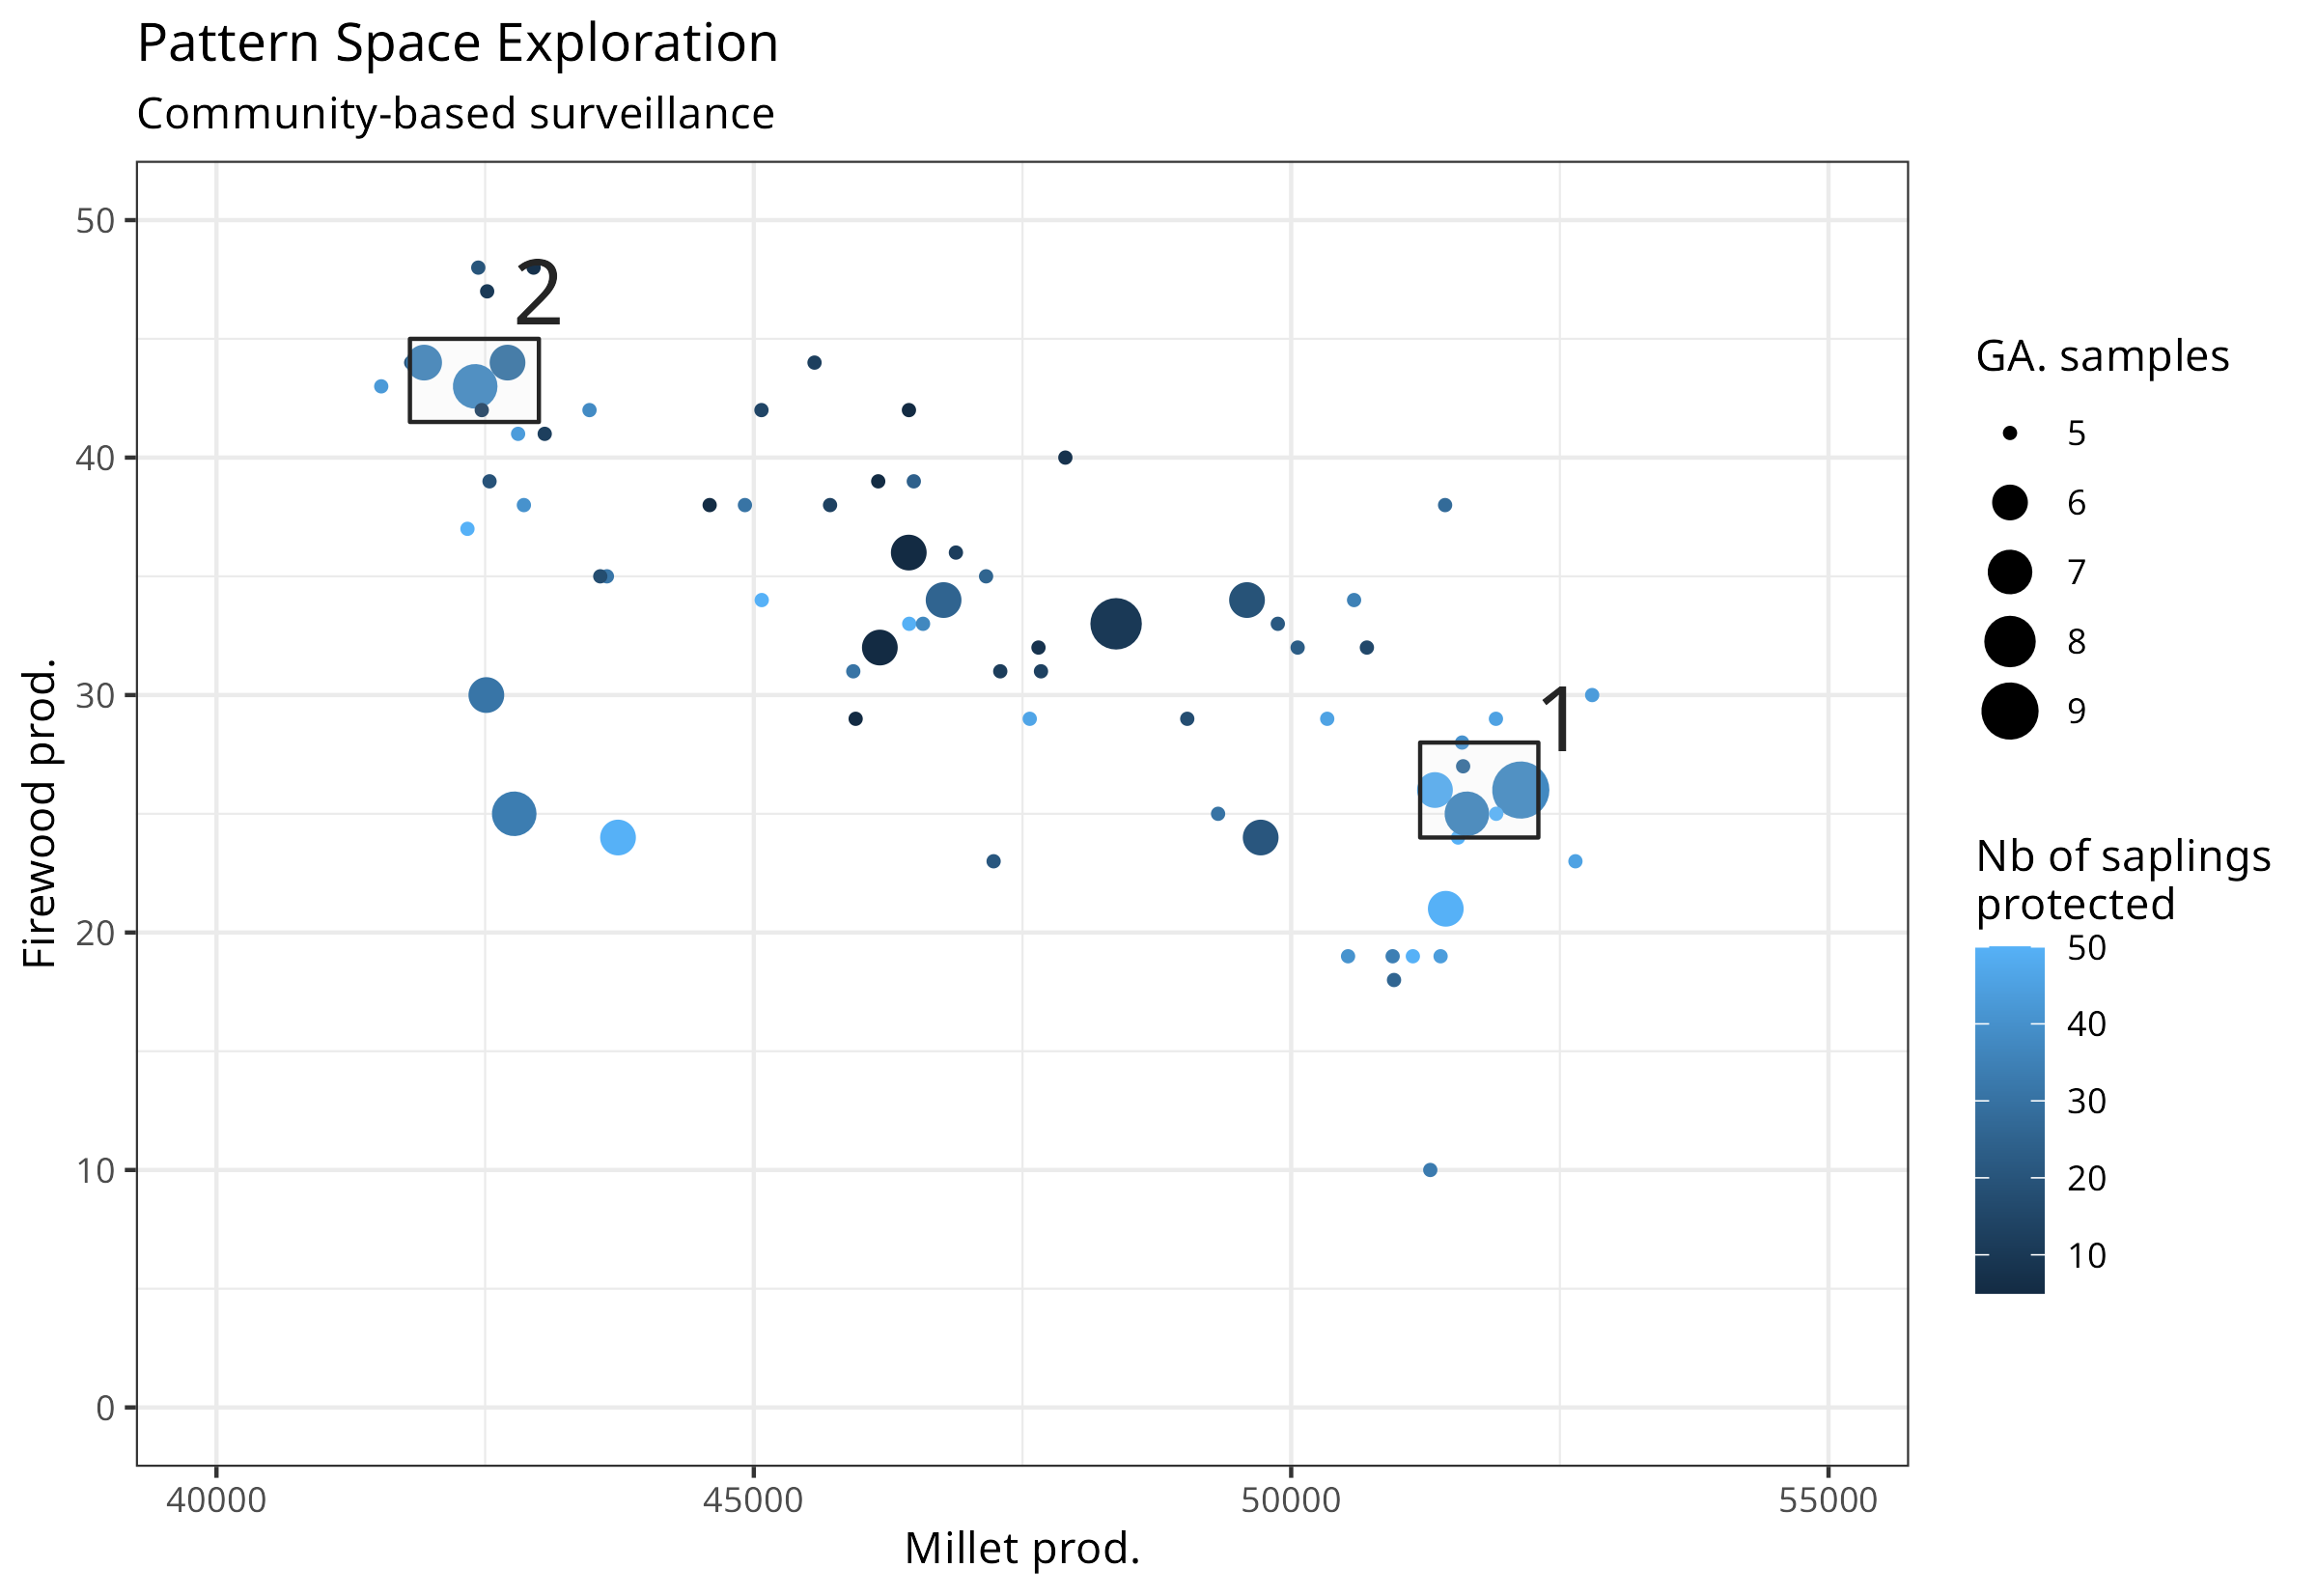
\includegraphics[width=1\linewidth]{./img/om_pse_sPop.png}
           \caption{}
           \label{fig:pseSPOP} 
        \end{subfigure}
        
        \begin{subfigure}[b]{0.85\textwidth}
           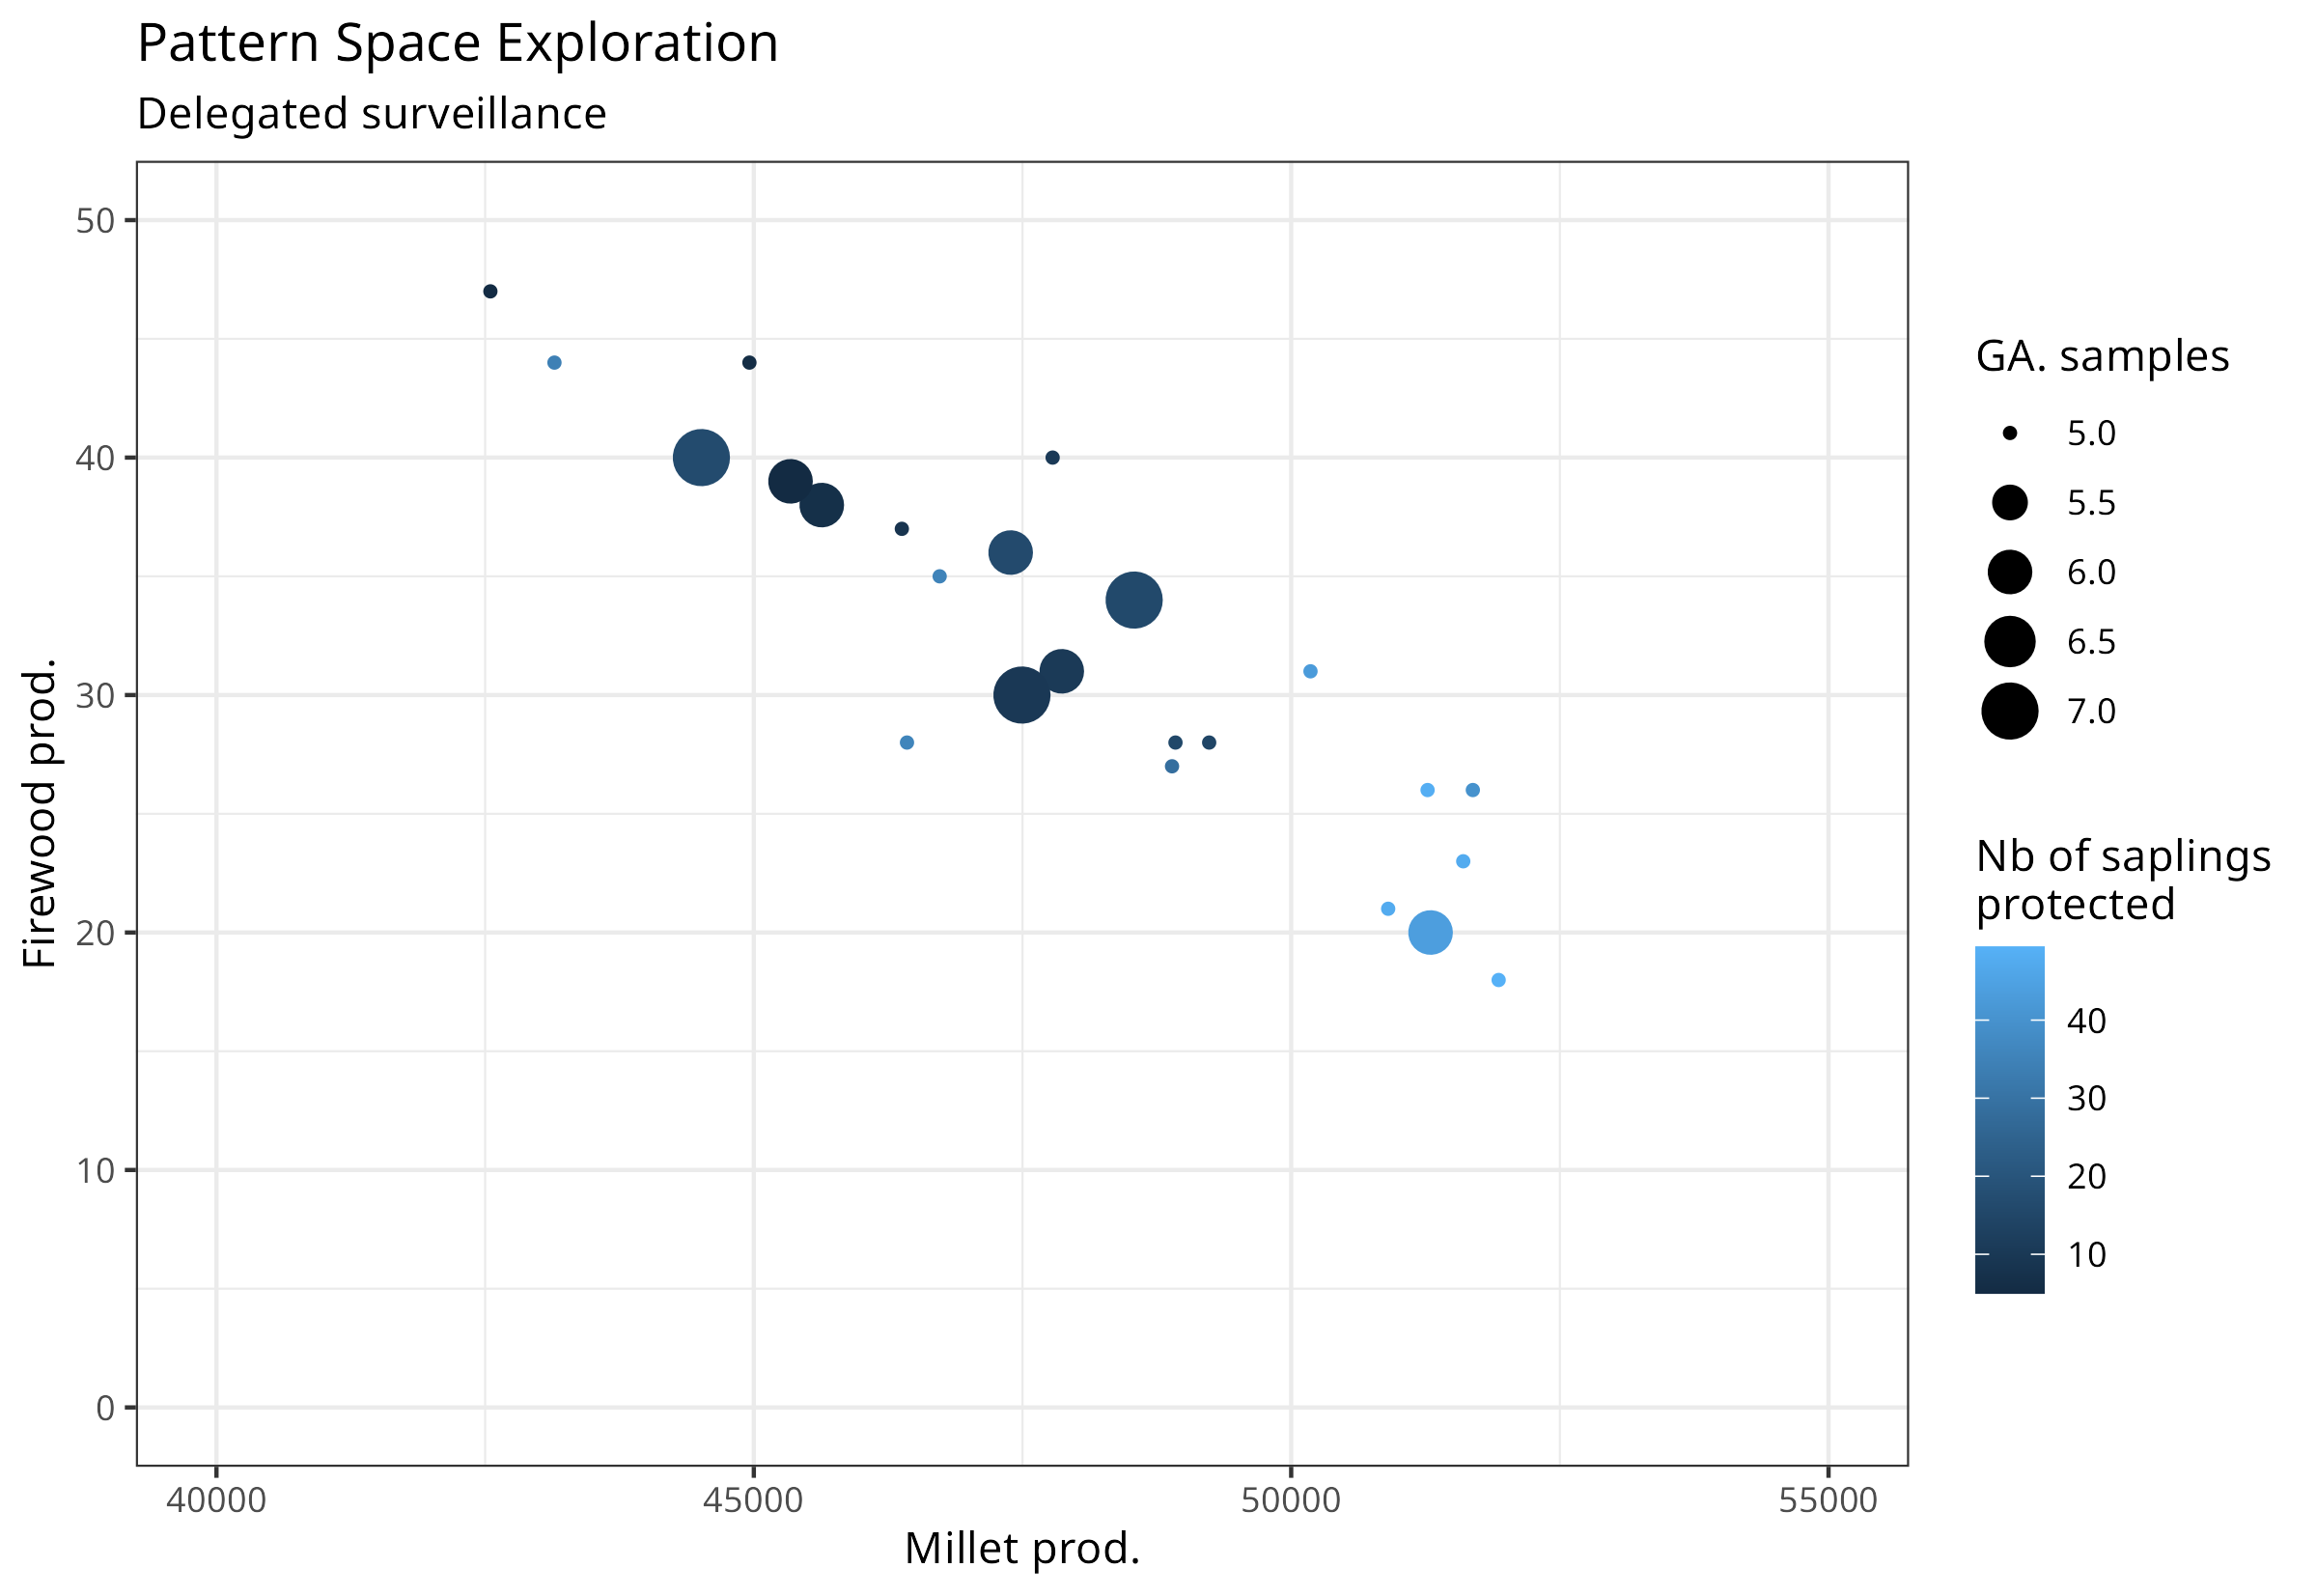
\includegraphics[width=1\linewidth]{./img/om_pse_sReprez.png}
           \caption{}
           \label{fig:pseSDELEG}
        \end{subfigure}
        
        \caption{PSE results for two different management scenarios: (a) community management and (b) management delegated to an external 'operator'. The size of the points (GA. sample) represents the number of times the algorithm reached this space during its evolution. The color of the points represents the number of young tree saplings that were protected. The x-axis denotes the millet production that was achievable, and the y-axis corresponds to the wood fuel extraction for cooking that was realized in the system. In figure (a), the two numbered squares, 1 and 2, represent the two contrasting situations that were discussed.}\label{fig:PSE}
    \end{figure}

 \subsection{Unexpected Yet Attainable: Surprising Results with Minimal Calculations}

 In the context of the co-construction of the simulation model, by integrating some basic indicators, we highlighted a fundamental issue that had never before been raised by the participants of the Living Lab as a major problem. By closely monitoring the total number of trees cut down, whether by herders for livestock, women for firewood, or farmers during their agricultural activities, a surprising trend emerged for the participants (see fig. \ref{fig:treeKilled}). This analysis revealed that farmers themselves significantly contribute to tree destruction, albeit in a somewhat silent manner. Specifically, this destruction often goes unnoticed because it manifests through the weeding of very young seedlings, carried out by farmers without their full awareness. This result was extensively discussed during the workshop, which allowed for the clarification of farming techniques to ensure that the translation into the model was accurate. This observation challenges some previous perceptions and raises essential questions regarding the management of tree resources within the community.

 \begin{figure}
    \centering
    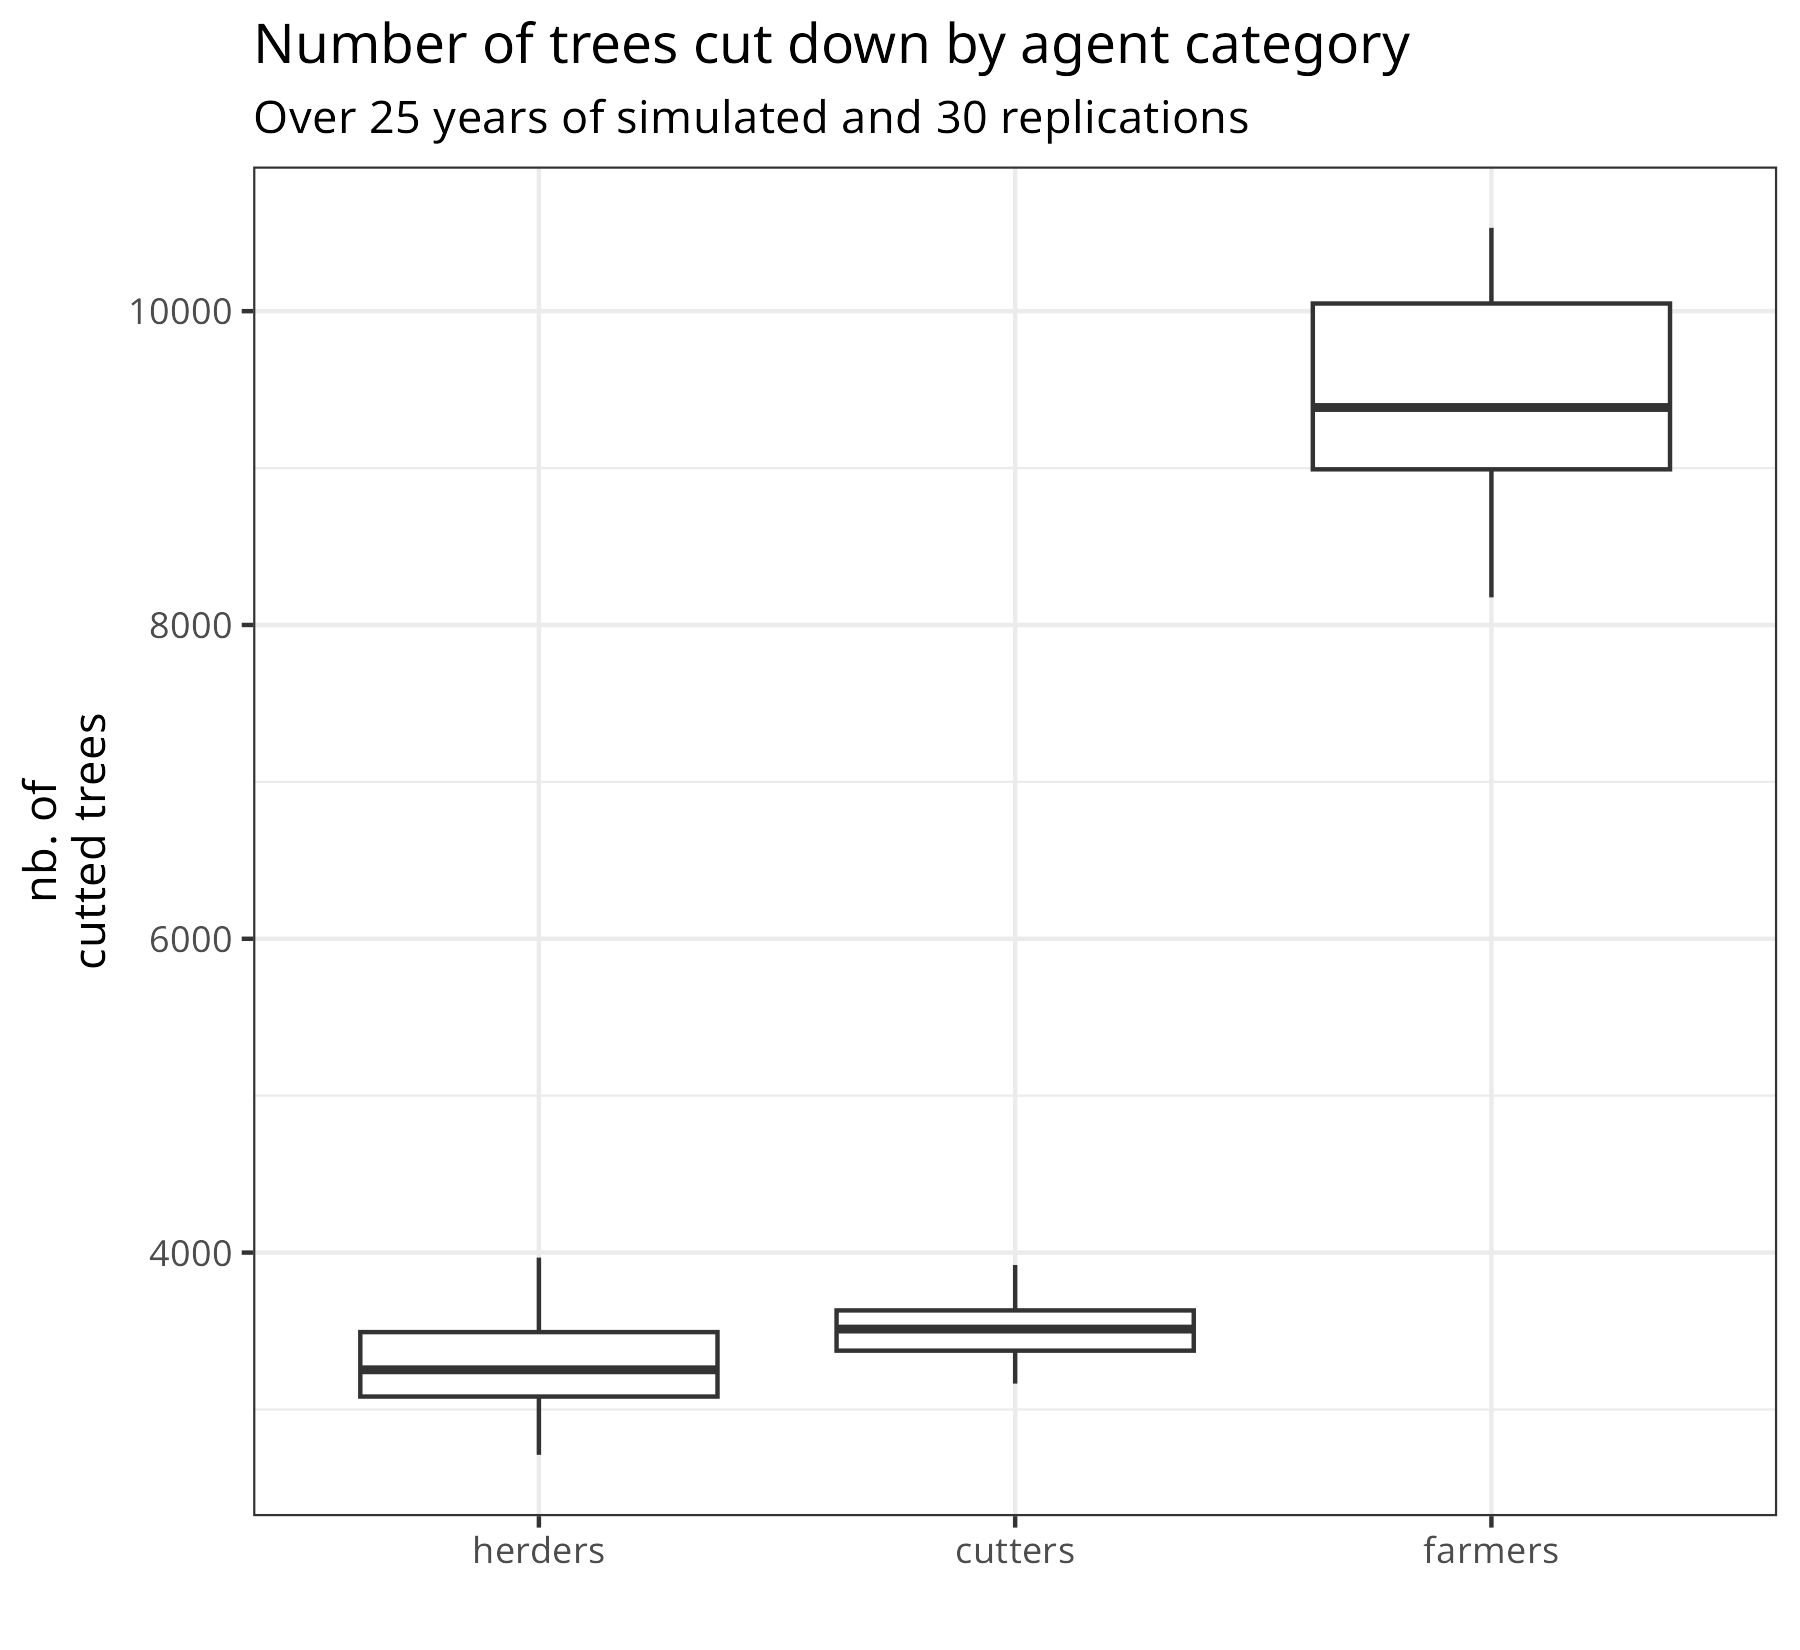
\includegraphics[width=\textwidth]{./img/rep_treeKilled.png}
    \caption{Boxplot showing the total number of trees cut down at the end of the simulation by resource user category. It is evident that farmers are responsible for the highest number of trees removed from the system across all categories. These results are based on 30 replications of the same parameter set.}
    \label{fig:treeKilled}
\end{figure}

% The results should describe the experiments performed and the findings observed. The results section should be divided into subsections to delineate different experimental themes. 
% \begin{itemize}
%     \item All data should be presented in the Results. No data should be presented for the first time in the Discussion. Data (such as from Western blots) should be appropriately quantified.
%     \item Subheadings must be either all complete sentences or all phrases. They should be brief, ideally less than 10 words. Subheadings should not end in a period. Your paper may have as many subheadings as are necessary.
%     \item Figures and tables must be called out in numerical order. For example, the first mention of any panel of Fig. 3 cannot precede the first mention of all panels of Fig. 2. The supplementary figures (for example, fig. S1) and tables (table S1) must also be called out in numerical order. 
% \end{itemize}

\section{Discussion}

As we outlined in the introduction, our purpose here is to support discussions and the ability of stakeholders to make concerted decisions by using companion modeling (ComMod). By adopting the "Different Modelling Purposes" from \parencite{edmonds_different_2019}, we position our intervention within two categories: illustration and social learning \parencite{sukthankar_kilt_2017}. Thus, we consider the process as a whole as the outcome \parencite{etienne_companion_2014}, leading the involved populations to re-examine their management practices of space and natural resources, in order to nurture the socio-spatial relationships that are under stress \parencite{selfa_politics_2008}.

The work we have conducted throughout this process allows us to discuss two dimensions: \textit{i)} the elements of the numerical results directly derived from the model co-constructed with the participants, and \textit{ii)} the transformative impact of the discussions that took place during the process, which have begun to change behaviors.

\subsection{Discussion of numerical Results}

Our global sensitivity analysis (tab. \ref{tab:saltelliCom} and \ref{tab:saltelliReprz}) revealed critical insights into the dynamics of community surveillance scenarios. Specifically, we found that the likelihood of community discussions regarding the importance of trees significantly influences both millet production (with a sensitivity index of 0.72) and the overall number of trees (sensitivity index of 0.59). These results underscore the crucial role of active participation and awareness within the community. They suggest that integrating structured discussions about tree preservation into major life events, like traditional rituals, and daily interactions could enhance the effectiveness of community-based natural resource management. By formalizing these discussions, communities can better understand and address the ecological and social implications of their traditional and current land use practices.\\

In scenarios where surveillance is delegated to forestry agents, the dynamics of resource management shift noticeably. While the time spent in the field and the likelihood of discussions on tree preservation continue to be significant, the introduction of external surveillance personnel brings additional dynamics into play. Our analysis indicates that the presence of these agents decreases the frequency of community meetings and the likelihood of reporting illegal activities, suggesting a shift towards a more controlled but potentially less community-involved management system. This shift was evident in our \textit{Pattern Space Exploration} (PSE) results (c.f. fig. \ref{fig:PSE}), highlighting changes in community dynamics under different surveillance regimes.\\

Our PSE analysis has unveiled a notable negative correlation between millet production and firewood harvesting, regardless of the regulatory approach employed. The simulations that reached the extremes of this model output space demonstrated that reducing firewood harvest not only protects more young plants but also significantly boosts millet yields. This finding suggests that policies aimed at reducing wood harvest could simultaneously enhance agricultural productivity and biodiversity conservation, offering a dual benefit to the communities involved.\\

\subsection{Driving Transformation Through Companion Modeling}


Our study has illuminated practical solutions through the use of community surveillance, which has shown improvements in either conservation or agricultural productivity goals. However, these benefits require a significant time investment from the community. Effective community surveillance not only demands involvement but also a commitment to ongoing dialogues and actions. This investment in time and effort needs to be supported by the community, recognizing the long-term benefits in fostering sustainable practices and enhanced resource management.\\

During our research, we identified a critical issue previously unnoticed by participants of the Living Lab : the significant impact of agricultural practices on tree destruction (c.f. fig. \ref{fig:treeKilled}). This destruction often goes unnoticed as it primarily involves the removal of young saplings during routine weeding, which is less dramatic than the felling of mature trees. The use of ploughs drawn by horses has eased the labor of farmers, yet has inadvertently led to the reduction of young trees. This oversight highlights the need for adapting agricultural practices to mitigate unintended environmental impacts.\\

%The discussion of our findings during the workshop sessions provided an opportunity to clarify agricultural techniques and ensure their accurate representation in our model. This process enhanced the model's relevance and precision, significantly improving participants' understanding of the dynamics at play. By refining these techniques in our simulations, we provided a clearer picture of how small-scale farming activities intersect with environmental conservation efforts.

The results of our study profoundly impacted the participants, prompting them to organize a community outreach day to share findings with neighboring villages. Recognizing that the protection of trees cannot be managed effectively at an individual or single-community scale, participants developed proposals for collective action during this deliberative session. This initiative reflects a strong community awareness and a commitment to extending the scope of conservation efforts beyond their immediate environment.

\section{Conclusion}


This research began by identifying the aspirations of local populations, from which we selected those we could feasibly address. Among these aspirations, the desire for a restored environment was paramount, manifesting in our efforts to increase tree populations, particularly of \textit{Faidherbia albida}.

Building on this aspiration, we collaborated with local communities through multiple workshops to develop an agent-based model. This model serves not just as a scientific tool but as a reflection of the community's perceived critical relationships and strategies necessary to achieve their environmental goals. This process melds scientific experimentation with co-construction and exploratory companion modeling, ensuring that the model's outcomes are deeply rooted in both empirical research and community insights.

The results of the model should be viewed within the trajectory of the community group, indicating that they encapsulate the relationships the group deemed essential for realizing their aspirations. These results highlight collective opportunities for improving tree counts in the area but also expose contradictions, such as the competing need for firewood for cooking.

This conflict suggests that in addition to protecting young saplings, it is crucial to promote alternatives to firewood, such as the use of improved stoves or \textit{Typha} charcoal. Protecting and increasing tree numbers in the area primarily requires supporting farmers to identify and preserve young saplings in the fields until they reach maturity.

Although the practice of marking young tree saplings for protection exists, it is not sufficiently adopted. The use of simulation to orchestrate the system of interrelationships that the actors co-constructed has been instrumental in raising awareness about the importance of collective action. This awareness has led to the organization of deliberation days on the subject with neighboring villages.

Engaging stakeholders in model exploration is an extremely powerful activity when aiming to encourage them to consider alternative futures. This participatory approach not only fosters a deeper understanding of the ecological and social dynamics at play but also empowers communities to actively participate in shaping their environmental futures.

\section*{Acknowledgments}

\subsection*{General} 
We warmly thank the residents of Diohine for their hospitality, with special thanks to: Aissatou Faye, Robert Diatte, Pierre Faye, Paul Sene, Ameth Paul Thiaw, Assane Diouf, Guedj Diouf, Nicolas Diouf, Ablaye Faye, Idrissa Faye, Maire-Hélène Ndjira Diouf, Seynabou Gakou, Joseph Sene, Ndeye Thiamal.

\subsection*{Author Contributions} 
Describe contributions of each author to the paper, using the first initial and full last name. 

``L. Broutin conceived the model and realize intervews.''

``E. Delay and L. Broutin animate multi-actor focus groups.''

``E. Delay assisted L. Broutin in the development of the model and conducte the HPC exploration.''

``E. Delay realize the first draft of this manuscript.''

``All authors contributed equally to 2nd version of the manuscript.''

\subsection*{Funding}

This work is part of the research and development project DSCATT (Dynamics of Soil Carbon Sequestration in Tropical and Temperate Agricultural Systems, https://dscatt.net/FR/index.html) co-funded by Agropolis Fondation [reference ID 1802-001] through the "Investissements d'avenir" program Labex Agro [ANR-10-LABX-0001-01] within the framework of I-SITE MUSE [ANR-16-IDEX-0006] and supported by the TOTAL Energies Foundation.

\subsection*{Conflicts of Interest}
The author(s) declare(s) that there is no conflict of interest regarding the publication of this article.

% \subsection*{Data Availability}
% A data availability statement is compulsory for all research articles. This statement describes whether and how others can access the data supporting the findings of the paper, including 1) what the nature of the data is, 2) where the data can be accessed, and 3) any restrictions on data access and why.

% If data are in an archive, include the accession number or a placeholder for it. Also include any materials that must be obtained through a Material Transfer Agreements (MTA). 

% \section*{Supplementary Materials}
% Describe any supplementary materials submitted with the manuscript (e.g., audio files, video clips or datasets). 

% Please group supplementary materials in the following order: materials and methods, figures, tables, and other files (such as movies, data, interactive images, or database files). 

% \medskip Example:
% Fig. S1. Title of the first supplementary figure.

% Fig. S2. Title of the second supplementary figure.

% Table S1. Title of the first supplementary table.

% Data file S1. Title of the first supplementary data file.

% Movie S1. Title of the first supplementary movie.

% \medskip
% Be sure to submit all supplementary materials with the manuscript and remember to reference the supplementary materials at appropriate points within the manuscript. We recommend citing specific items, rather than referring to the supplementary materials in general, for example: ``See Figures S1-S10 in the Supplementary Material for comprehensive image analysis.''

% A link to access the supplementary materials will be provided in the published article.

% Supplementary Materials may include additional author notes—for example, a list of group authors.

% \section*{Guidelines for References}

% There is only one reference list for all sources cited in the main text, figure and table legends, and Supplementary Materials. Do not include a second reference list in the Supplementary Materials section. Include references cited only in the Supplementary Materials at the end of the reference section of the main text; reference numbering should continue as if the Supplementary Materials are a continuation of the main text. References cited only in the Supplementary Materials section are not counted toward length guidelines.

% Authors are responsible for ensuring that the information in each reference is complete and accurate.

% DOIs, if available, should be included for each reference.

% Please do not include any extraneous language such as explanatory notes as part of a reference to a given source. The Journal of Remote Sensing prefers that manuscripts do not include end notes; if information is important enough to include, please put into main text.  If you need to include notes, please explain why they are needed in your cover letter to the editor.

\printbibliography

\end{document}
